\section[AppofDiff]{Application of Differential Calculus}
\begin{frame}{Slope of tangent lines}

\begin{onlyenv}<+>

\begin{example}
Find the equations of the tangent and normal to the curve of $f\left(x\right)=x^{3}-3x^{2}$
at the point $\left(1,-2\right)$.
\end{example}



\begin{example}
Find the equation of the tangent to $x^{2}y-x=y^{3}-8$ at the point
where $x=0$.
\end{example}

\end{onlyenv}



\begin{onlyenv}<+>

\begin{example}
Find the coordinates of any point on the curve of $y^{2}-4xy=x^{2}+5$
for which the tangent is horizontal.
\end{example}



\begin{example}
(slope of parametric curves) Find the equation of the tangent to $F\left(t\right)=\left(\cos t,2\sin^{2}t\right)$
at the point where $t=\frac{\pi}{3}$.
\end{example}



\begin{example}
(slope of polar curves) Find the slope of the cardioid $r=2\left(1+\cos\theta\right)$
at $\theta=\frac{\pi}{6}$. Where is the tangent to the curve horizontal?
\end{example}

\end{onlyenv}

\end{frame}

\begin{frame}{Average and instantaneous rates of change}

\begin{onlyenv}<1>

\begin{itemize}
\item Average rate of change
\[
\frac{f\left(a+h\right)-f\left(a\right)}{h}\,,\quad\frac{f\left(b\right)-f\left(a\right)}{b-a}\,.
\]

\item Instantaneous rate of change/derivative
\[
\lim_{h\to0}\frac{f\left(a+h\right)-f\left(a\right)}{h}\,,\quad\lim_{b\to a}\frac{f\left(b\right)-f\left(a\right)}{b-a}\,.
\]

\end{itemize}
\end{onlyenv}



\begin{onlyenv}<2>

\begin{example}
Let $G\left(t\right)=400\left(15-t\right)^{2}$ be the number of gallons
of water in a tank $t$ minutes after an outlet pipe is opened. Find
the average rate of drainage during the first $5$ minutes and the
rate at which the water is running out at the end of $5$ minutes.
\end{example}

\end{onlyenv}

\end{frame}

\begin{frame}{Monotonicity, concavity and local extrema}

\begin{onlyenv}<1>


\begin{center}
\begin{tabular}{|>{\raggedleft}p{0.15\columnwidth}|>{\raggedright}p{0.23\columnwidth}|>{\raggedright}p{0.23\columnwidth}|>{\raggedright}p{0.23\columnwidth}|}
\hline 
 & {\small{}$f$} & {\small{}$f'$} & {\small{}$f''$}\tabularnewline
{\small{}$>0$} & {\small{}positive} & {\small{}increasing} & {\small{}concave up}\tabularnewline
{\small{}$<0$} & {\small{}negative} & {\small{}decreasing} & {\small{}concave down}\tabularnewline
{\small{}$=0$} & {\small{}roots} & {\small{}possible local extremes} & {\small{}possible inflection point}\tabularnewline
{\small{}not exist} & {\small{}out of domain} & {\small{}possible local extremes} & {\small{}possible inflection point}\tabularnewline
\hline 
\end{tabular}
\par\end{center}
\begin{itemize}
\item For the possible extremes/inflection points, you need to check the
trend around that point. Always remember the examples of $x^{3}$
and $x^{4}$.
\item The points at which $f'$ equals $0$ or does not exist are called
\alert{critical points}.
\end{itemize}
\end{onlyenv}



\begin{onlyenv}<2,3>

\begin{example}
Find all the local maximum, minimum, inflection points on the graph
of $f\left(x\right)=x^{3}-5x^{2}+3x+6$ and sketch the graph.
\end{example}
\uncover<3>{
\begin{example}
p241-3, 4, 5; p242-11 to 14, 40, 46; p252-18
\end{example}
}
\end{onlyenv}

\end{frame}

\begin{frame}{Global minimum or maximum}

Based on the analysis of local/relative extremum, take the values
at end points into account.
\begin{example}
p272-17 to 20; p273-43, 44
\end{example}

\end{frame}

\begin{frame}{Optimization}

\begin{onlyenv}<1-6>
\begin{enumerate}[<+->]
\item Find out the \alt<+->{dependent variable}{quantity we want to optimize};
\item Find out the \alt<+->{independent variables}{factor that changes the quantity we study};
\item Establish a function between dependent and independent variables;
\item Find out the (usually global) maximum/minimum. Remember to use the correct domain.
\end{enumerate}
\end{onlyenv}

\begin{onlyenv}<+>

\begin{example}
The region in the first quadrant bounded by the curves of $y^{2}=x$
and $y=x$ is rotated about the $y$-axis to form a solid. Find the
area of the largest cross section of this solid that is perpendicular
to the $y$-axis.

\begin{center}
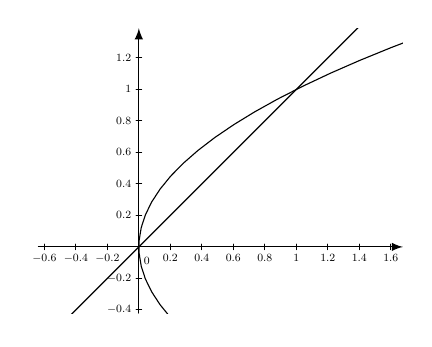
\begin{tikzpicture}[line cap=round,line join=round,>=latex,x=4.0cm,y=4.0cm,scale=0.5,transform shape]
\draw[->,color=black] (-0.6382410397208873,0.) -- (1.6766681092950013,0.);
\foreach \x in {-0.6,-0.4,-0.2,0.2,0.4,0.6,0.8,1,1.2,1.4,1.6}
\draw[shift={(\x,0)},color=black] (0pt,2pt) -- (0pt,-2pt) node[below] {\footnotesize $\x$};
\draw[->,color=black] (0.,-0.42090839657235085) -- (0.,1.388633262165417);
\foreach \y in {-0.4,-0.2,0.2,0.4,0.6,0.8,1,1.2}
\draw[shift={(0,\y)},color=black] (2pt,0pt) -- (-2pt,0pt) node[left] {\footnotesize $\y$};
\draw[color=black] (0pt,-10pt) node[right] {\footnotesize $0$};
\clip(-0.6382410397208873,-0.42090839657235085) rectangle (1.6766681092950013,1.388633262165417);
\draw [samples=50,domain=-2.0:2.0)] plot[rotate around={-90.:(0.,0.)}] (\x,{(\x)^2});
\draw [domain=-0.6382410397208873:1.6766681092950013] plot(\x,\x);
\end{tikzpicture}
\par\end{center}

\end{example}

\end{onlyenv}



\begin{onlyenv}<+>

\begin{example}
The volume of a cylinder equals $V$ cubic inches, where $V$ is a
constant. Find the proportions of the cylinder that minimize the total
surface area.
\end{example}



\begin{example}
p286-51
\end{example}

\end{onlyenv}

\end{frame}

\begin{frame}{Motion along a line}
\begin{onlyenv}<1>
If the position/displacement of the particle $P$ on the line at time $t$ is modeled by
\[
s=f\left(t\right)\,.
\]
Then
\[
v=\frac{\mathrm{d}s}{\mathrm{d}t}\,,a=\frac{\mathrm{d}v}{\mathrm{d}t}=\frac{\mathrm{d}^{2}s}{\mathrm{d}t^{2}}\,.
\]
\end{onlyenv}

\begin{onlyenv}<2>
\begin{itemize}
\item If $v>0$, then $P$ is moving to the right and its position $s$
is increasing;
\item If $v<0$, then $P$ is moving to the left and its position $s$ is
decreasing;
\item If $a$ and $v$ have different signs, then the speed is decreasing;
\item If $a$ and $v$ have the same sign, then the speed is increasing.
\end{itemize}
\end{onlyenv}

\begin{onlyenv}<3>
\begin{example}
If the law of motion is
\[
s=2t^{3}-9t^{2}+12t-4
\]
where $t\ge0$.
\begin{enumerate}
\item Find all $t$ for which the position $s$ is increasing.
\item Find all $t$ for which the velocity is increasing.
\item Find all $t$ for which the speed of the particle is increasing.
\item Find the speed when $t=\frac{3}{2}$.
\item Find the total distance traveled between $t=0$ and $t=4$.
\end{enumerate}
\end{example}
\end{onlyenv}
\end{frame}

\begin{frame}{Motion along a curve}
\begin{onlyenv}<1>
The position of a particle moving on the plane is described by the
coordinates
\[
\vec{s}=\left(x\left(t\right),y\left(t\right)\right)\,.
\]
Then
\[
\vec{v}=\left(\frac{\mathrm{d}x}{\mathrm{d}t},\frac{\mathrm{d}y}{\mathrm{d}t}\right)\,.
\]
Recall that the slope of the tangent line of the parametric curve
is given by
\[
\frac{\mathrm{d}y}{\mathrm{d}x}=\frac{y'}{x'}=\frac{\frac{\mathrm{d}y}{\mathrm{d}t}}{\frac{\mathrm{d}x}{\mathrm{d}t}}\,.
\]
This is $\tan\theta$ where $\theta$ gives you the direction of the
velocity vector.

\alert{What is the acceleration for the particle? }
\end{onlyenv}

\begin{onlyenv}<2>
\begin{example}
A particle moves according to the equations $x=3\cos t$, $y=2\sin t$.
\begin{enumerate}
\item Find a single equation in $x$ and $y$ for the path of the particle
and sketch the curve.
\item Find the velocity and acceleration vectors at any time $t$.
\item Find the position, velocity and acceleration at $t=\frac{\pi}{6}$
and sketch them.
\item Find the speed of the particle and the magnitude of its acceleration
in 3.
\item When is the speed a maximum? minimum?
\end{enumerate}

\end{example}

\end{onlyenv}

\end{frame}

\begin{frame}{Tangent line approximation}

\begin{onlyenv}<1,2>


For a function $y=f\left(x\right)$, if we have known $f\left(a\right)$
and $f'\left(a\right)$, then we can approximate the value of $f\left(x\right)$
for $x$ near $a$, by the formula
\[
f\left(x\right)\approx f\left(a\right)+f'\left(a\right)\left(x-a\right)\,.
\]
Recall that if we also know higher order derivatives, we can get more
accurate approximation by using
\[
f\left(x\right)\approx f\left(a\right)+f'\left(a\right)\left(x-a\right)+\frac{f''\left(a\right)}{2!}\left(x-a\right)^{2}+\cdots\,,
\]
which is called \uncover<2>{Taylor series.}

\end{onlyenv}



\begin{onlyenv}<3>

\begin{example}
Find the formulae for approximation of the following functions around
given points
\begin{enumerate}
\item $\sin x$ at $a=0$;
\item $\cos x$ at $a=\frac{\pi}{2}$;
\item $2x^{3}-3x$ at $a=1$;
\item $\sqrt{1+x}$ at $a=8$.
\end{enumerate}

\end{example}

\end{onlyenv}



\begin{onlyenv}<4>

\begin{example}
Find by approximately how much the area of a circle changes when the
radius increases from $3$ to $3.01$ inches.
\end{example}

\end{onlyenv}

\end{frame}

\begin{frame}{Related rates}

\begin{onlyenv}<1>

\begin{example}
If one leg $AB$ of a right triangle increases at the rate of $2$
inches per second, while the other leg $AC$ decreases at $3$ inches
per second, find how fast the hypotenuse is changing when $AB=6$
feet and $AC=8$ feet.

\begin{center}
\definecolor{qqwuqq}{rgb}{0.,0.39215686274509803,0.}
\definecolor{qqqqff}{rgb}{0.,0.,1.}
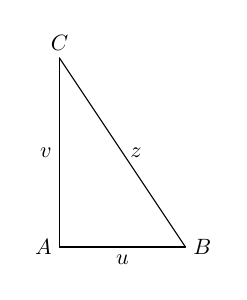
\begin{tikzpicture}[scale=0.8, transform shape,line cap=round,line join=round,>=latex,x=1.0cm,y=1.0cm]
\draw (0,0)--(2,0) node [midway, below] {$u$};
\draw (0,0)--(0,3) node [midway, left] {$v$};
\draw (2,0)--(0,3) node [midway, right] {$z$};
\node [left] at (0,0) {$A$};
\node [right] at (2,0) {$B$};
\node [above] at (0,3) {$C$};
\end{tikzpicture}
\par\end{center}

\end{example}

\end{onlyenv}



\begin{onlyenv}<2>

\begin{enumerate}
\item In these questions, you will always find several rates $u'$, $v'$
etc. given to you and one unknown rate $F'$.
\item Find out of what quantities these rates are, i.e., $u$ and $v$ etc.
\item Relate $F$ and $u$, $v$ by a function.
\item Differentiate this function with respect to time $t$ or whatever
the fundamental variable is. Then you get a relation between $F'$
and $u'$, $v'$ etc.
\end{enumerate}
\end{onlyenv}



\begin{onlyenv}<3>

\begin{example}
The diameter and height of a paper cup in the shape of a cone are
both $4$ inches, and water is leaking out at the rate of $\frac{1}{2}$
cubic inch per second. Find the rate of which the water level is dropping
when the diameter of the surface is $2$ inches.
\end{example}

\end{onlyenv}

\end{frame}



